\subsection{Global Declarations}
\subsubsection{System Parameters}

\begin{table} [H]
    \begin{tabu} to \textwidth {|X|X[2]|}
        \hline
        \textbf{Parameter}              & \textbf{Description} \\  \hline
        nStations                       & Number of stations in the system \\  \hline
        nTrains                         & Number of trains in the system \\    \hline
        chargingSpeed                   & A multiplier for the battery charging speed \\    \hline
        journeyDischargeMultiplier      & A multiplier for the battery discharge during the journey \\  \hline
        waitingDischargeMultiplier      & A multiplier for the battery discharge during the waiting \\  \hline
        MIN\_TIME\_PER\_STATION         & Lower bound to allow passengers to get on and off the train \\    \hline
        trainSpeed                      & Trains' speed \\   \hline
        stationNumOfTracks              & Array with the number of tracks of each station \\   \hline
        railLine\_distance              & Matrix containing the distance between stations \\    \hline
        railLine\_delay                 & Matrix containing the maximum delay between stations \\   \hline
    \end{tabu}
\end{table}
\bigskip

\subsubsection{System Variables}
\begin{table} [H]
    \begin{tabu} to \textwidth {|X|X[2]|}
    \hline
    \textbf{Variable}          & \textbf{Description} \\  \hline
    trainStation                & Array with the current station of each train \\  \hline
    trainDestination            & Array with the destination of each train \\   \hline
    nextStop                    & Array with the next station of each train \\  \hline
    stationFreeTracks           & Array with the current number of free tracks of each station \\   \hline
    chargeOfTrain               & Array with the current charge of each train battery \\    \hline
    \end{tabu}
\end{table}
\bigskip

\subsubsection{System Channels}
\begin{table} [H]
    \begin{tabu} to \textwidth {|X|X[2]|}
    \hline
    \textbf{Channel}          & \textbf{Description} \\  \hline
    exitTrain                   & Channels through which a train inform its current station that it is leaving \\  \hline
    full                        & Channels through which a station communicate to an incoming train that it has no available tracks\\  \hline
    allowedIn                   & Channels through which a station grant the access to a train that is waiting \\ \hline
    arrived                     & Channels through which a train inform its next station that it is arrived\\ \hline
    \end{tabu}
\end{table}

\newpage

\subsection{Templates}
\subsubsection{Station}
\begin{figure}[H]
    \centering
    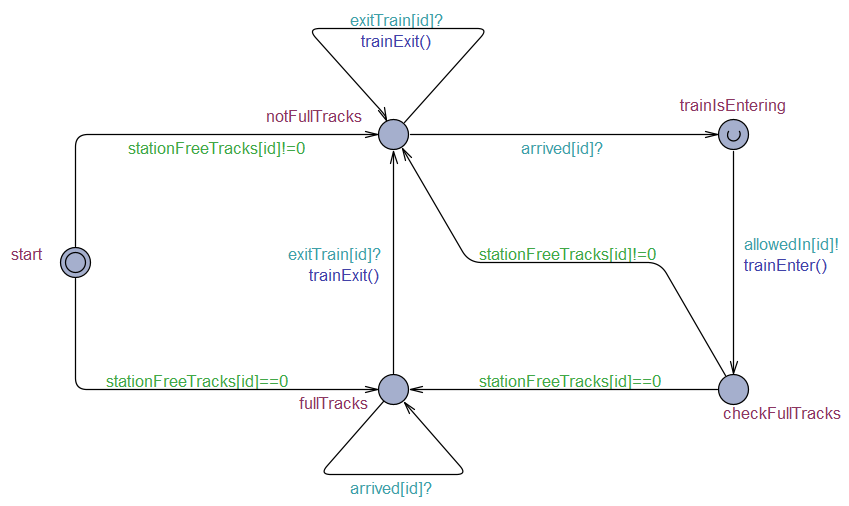
\includegraphics[scale=0.9]{images/stationTemplate.png}
\end{figure}

\begin{itemize}
    \item \textbf{start: }this is the initial state of the Station Template. In case the number of available
            tracks is equal to zero the next state is notFullTracks, otherwise the next state is \emph{fullTracks}.
    \item \textbf{notFullTracks: }when this state receives a message on the \emph{exitTrain} channel, it updates his 
            \emph{stationFreeTracks} variable and the current state doesn't change. Upon receiving a message on the 
            \emph{arrived} channel the current state moves to \emph{checkFreeTracks} state.
    \item \textbf{fullTracks: }when this state receives a message on the \emph{arrived} channel the current state doesn't change. 
            Instead, if this state receives a message on the \emph{exitTrain} channel, it updates his \emph{stationFreeTracks} 
            variable and the current state moves to \emph{notFullTracks} state.
    \item \textbf{trainIsEntering: }this is an urgent state created to describe when a train is joining the station.
    \item \textbf{checkFullTracks: }this state is reached immediately after the update of the \emph{stationFreeTracks} variable
            and checks if the station has available tracks. In this case the current state becomes \emph{notFullTracks},
            otherwise it becomes \emph{fullTracks}.
\end{itemize}
\newpage

\subsubsection{Train}
\begin{figure}[H]
    \centering
    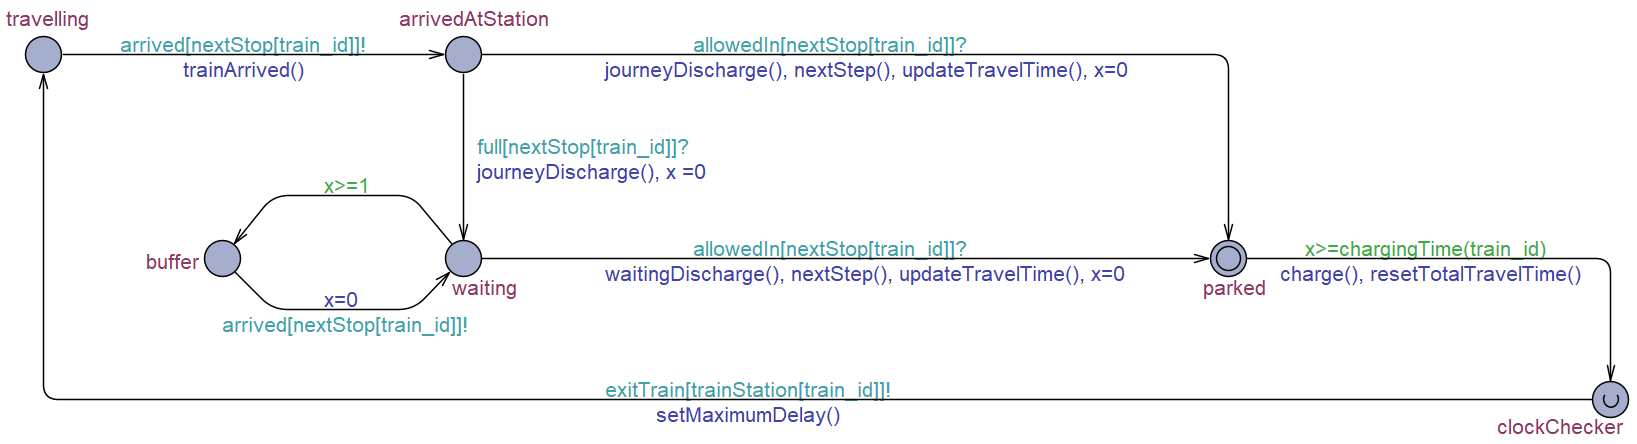
\includegraphics[scale=0.56]{images/trainTemplate.png}
\end{figure}

\begin{itemize}
    \item \textbf{parked: }this is the initial state of the Train Template. It represents the situation in which the train is
            stopped in a station. The current state changes only if the clock is greater or equal to the needed charging time.
            Before the current state changes in \emph{clockChecker} we compute the \emph{charge} method that increases the
            train battery linearly with the time spent in the station.
    \item \textbf{clockChecker: }this is an urgent state created to send a message on \emph{exitTrain} channel and to set
            the maximum delay to reach the next station.
    \item \textbf{travelling: }this state represents the situation in which the train left the previous station and heads to
            the next one. Before reaching the next station, we send a message on \emph{arrived} channel to inform the station
            of the arrival and update train's current station.
    \item \textbf{arrivedAtStation: }this state checks if the train has to wait before entering or if it is allowed to join 
            the station. In the first case the current state becomes \emph{waiting} after receiving a message on \emph{full}
            channel, otherwise the system comes back to the initial state after receiving a message on \emph{allowedIn} channel.
            Before reaching one of the next state we compute the \textit{journeyDischarge} method that decreases
            the train battery linearly with the travel time.
    \item \textbf{waiting: }this is the state in which the train waits until the station, throw \emph{allowedIn} channel,
            allows him to join. Before entering the station we compute the \textit{waitingDischarge} method that decreases
            the train battery linearly with the waiting time.
    \item \textbf{waiting-buffer: }this is a snippet of Train Template that describes the loop in which the train is while
            waiting to be allowed to join the next station. In this loop we send a message through \emph{arrived} channel
            to the station every clock time unit.
            \begin{figure}[H]
                \centering
                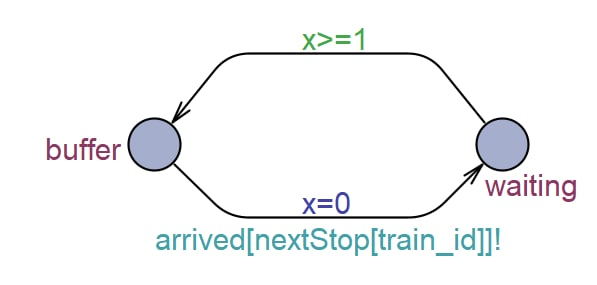
\includegraphics[scale=0.56]{images/bufferSnippet.png}
            \end{figure}
\end{itemize}

\newpage

\begin{table} [H]
    \begin{tabu} to \textwidth {|X|X[3.5]|}
    \hline
    \textbf{Train local variables}              & \textbf{Description} \\  \hline
    x                       & This is the clock used to temporalize the system \\  \hline
    totalTravelTime         & An int that represents the overall time to reach the next station \\    \hline
    parkedTime              & An int that represents the time spent in a station \\    \hline
    travelTime              & An int that represents the time spent in the journey \\  \hline
    waitingTime             & An int that represents the time wasted until the station authorizes the access \\  \hline
    actualMaximumDelay      & An int used to save the maximum delay allowed to reach the next station \\    \hline
    \end{tabu}
\end{table}

\newpage
